\documentclass[11pt]{article}
\usepackage{geometry}
\geometry{
 a4paper,
 total={170mm,257mm},
 left=20mm,
 top=20mm,
 }
\usepackage[french]{babel}
\usepackage[T1]{fontenc}
\usepackage[utf8]{inputenc}
\usepackage{lmodern}
\usepackage{graphicx}
\usepackage{amssymb}
\usepackage{microtype}
\usepackage[colorlinks=true,
            linkcolor=red,
            urlcolor=blue,
            citecolor=blue]{hyperref}
\title{Simulation de fluides}
\author{Raoelisolonarivony - MISA M2}
\date{Décembre 2016}
\setlength{\parindent}{2em}
\setlength{\parskip}{1em}
\linespread{1.3}
\usepackage{fancyhdr}
\pagestyle{fancy}

\renewcommand{\headrulewidth}{0.5pt}
\fancyhead[L]{RAOELISOLONARIVONY - MISA M2 - \textit{Simulation de fluides}}
\fancyhead[C]{}
\fancyhead[R]{Décembre 2016}

\begin{document}

\maketitle

\section{Introduction}

Le monde est rempli de scènes et d’évènements incroyables impliquant les fluides. Par exemple, les tempêtes de sable, les vagues de l'océan, les colonnes de feu, les coulées de lave, les explosions, tant de phénomènes naturels difficiles à reproduire matériellement, tant leur simulation par ordinateur s'avère toute indiquée. La simulation des fluides suit un modèle de générateurs physiques: la compréhension du mouvement d'un fluide dans une animation n'est pas possible sans connaître les bases mathématiques et physiques qui régissent son déplacement et ses interactions avec son environnement. Cette note comprend trois parties: les bases mathématiques et physiques concernant l'écoulement des fluides, la visualisation des fluides,  et pour finir la simulation de la fumée.

\section{Les équations des fluides}

\subsection{Les équations de Claude-Louis Navier et Georges Gabriel Stokes}

Les fameuses
\footnote{La résolution des équations de Navier-Stokes constitue l'un des problèmes du prix du millénaire. \url{http://www.claymath.org/millennium-problems/navier–stokes-equation}}
équations de Navier-Stokes gouvernent le mouvement d'écoulement d'un fluide dit incompressible. C'est un ensemble d'équations aux dérivées partielles (EDP):
	\begin{eqnarray}\label{equation/navier-stokes-1}
	\frac{\partial \overrightarrow{u}}{\partial t} + (\overrightarrow{u} . \nabla ) \overrightarrow{u} + \frac{1}{\rho} \nabla p & = & \overrightarrow{g} + \nu \nabla . \nabla \overrightarrow{u} \\
	\label{equation/navier-stokes-2}
\nabla . \overrightarrow{u} & = & 0
	\end{eqnarray}

\begin{itemize}
	\item Le symbole $ \overrightarrow{u} $ représente la vitesse du fluide.
	\item $  \rho $ est la masse volumique du fluide. Pour l'eau, $ \rho \approx 1000\,kg.m^{-3} $ tandis que pour l'air elle est de l'ordre de $ 1,3\,kg.m^{-3} $.
	\item La "\textbf{pression}" \textit{p} est la force exercée par le fluide sur une unité de surface.
	\item Le symbole \overrightarrow{g} est l'accélération de la pesanteur.
	\item $\nu$ est la "\textbf{viscosité cinématique}". Elle mesure à quel point un fluide peut se déformer durant son écoulement, et sa force de résistance (frottement) par rapport à une déformation. Par exemple le pois a une plus grande viscosité que l'alcool.
\end{itemize}

La première équation différentielle (\ref{equation/navier-stokes-1}) est associée au mouvement du fluide et aux forces qui s'exercent sur lui, en bref l'évolution du fluide au cours du temps. La seconde équation (\ref{equation/navier-stokes-2}) est la "\textbf{condition d'incompressibilité}". Il est utile de décortiquer ces équations pour en saisir le sens.

L'ensemble du fluide peut être modélisée comme un système de particules libres de se déplacer les unes par rapport aux autres. Chaque particule a une masse \textit{M}, un volume \textit{V} et une vitesse \overrightarrow{u}. Le bilan des forces appliquées sur la particule conjugué avec l'équation de Newton $ \overrightarrow{F} = m\, \overrightarrow{a} $ donne son accélération. Or par définition, l'accélération est $\overrightarrow{a} = \frac{D \overrightarrow{u}}{Dt}$ alors l'équation de Newton devient: $\overrightarrow{F} = m\, \frac{D \overrightarrow{u}}{Dt}$.

Parmi les forces s'exerçant sur la particule, la force de la \textbf{gravité} $ m\overrightarrow{g} $ est la plus évidente. 

Les particules du fluide s'exercent entre elles la force de la \textbf{pression}. Si une particule est soumise à une pression égale dans toutes les directions, la somme des forces sera nulle. En revanche, si une haute pression appuie sur un côté particulier de la particule, il y a une variation de pression sur la particule. Cette variation se calcule par le \textit{gradient de pression} précédé du signe moins: $ - \overrightarrow{\nabla} p $.
L'intégrale de cet élément sur le volume entier du fluide donne la force de pression. Ou bien par approximation, il est possible de simplement multiplier par le volume $V$. En réalité, la pression garde le volume du fluide constant.

L'autre force exercée par une particule est la force de \textbf{viscosité}. Un fluide visqueux tend à résister à la déformation. C'est une force qui pousse la particule avec comme vitesse la moyenne des vitesses des particules voisines, c'est-à-dire qu'elle cherche à minimiser les différences de vitesses entre les particules voisines dans le fluide. L'opérateur différentiel \textit{laplacien} $ \nabla . \nabla \overrightarrow{u}$ mesure à quelle proportion une quantité, ici la vélocité, varie autour de la moyenne. L'intégration de cette valeur sur le volume entier donne la force due à la viscosité. Le "\textit{coefficient de viscosité dynamique}" noté $ \mu $ est relié à cette force.

En regroupant toutes les forces et en remplaçant $\overrightarrow{F}$ dans l'équation de Newton, le mouvement suit l'équation suivante:
	\begin{eqnarray}\label{equation/newton-3}
	m\overrightarrow{g} - V \overrightarrow{\nabla} p + V \mu \,\,\nabla\!.\!\nabla \overrightarrow{u} & = & m \frac{D \overrightarrow{u}}{Dt}
	\end{eqnarray}
L'approximation du fluide avec un nombre fini de particules introduit des erreurs. Il faut réduire la taille des particules en la faisant tendre vers zéro tandis que le nombre de particules doit tendre vers l'infini. L'équation du mouvement de la particule est affecté par ces limitations puisque la masse \textit{m} et le volume \textit{V} vont tendre vers zéro.
Pour pallier ce problème, il faut diviser membre à membre l'équation (\ref{equation/newton-3}) par le volume, en tenant compte que la masse volumique $ \rho $ = $ \frac{m}{V} $. L'équation devient:
	\begin{eqnarray}
	\rho\overrightarrow{g} - \nabla p + \mu \,\,\nabla\!.\!\nabla \overrightarrow{u} & = & \rho \frac{D \overrightarrow{u}}{Dt}
	\end{eqnarray}
En divisant ensuite par la masse volumique $ \rho $ et comme la viscosité cinématique est égale à $ \nu = \frac{\mu}{\rho} $ (quantifie sa capacité à s’épancher), l'équation devient:
	\begin{eqnarray}
	\overrightarrow{g} - \frac{1}{\rho}\nabla p + \nu \,\,\nabla\!.\!\nabla \overrightarrow{u} & = & \frac{D \overrightarrow{u}}{Dt}
	\end{eqnarray}

L'équation (\ref{equation/navier-stokes-1}) est sensiblement retrouvée. En fait, l'utilisation de la dérivée totale $ \frac{D\overrightarrow{u}}{Dt} $ est plus importante pour la synthèse d'image et nous conduit à des méthodes de résolutions numériques de l'équation. Pour expliciter cette importance de la dérivée totale $ \frac{D\overrightarrow{u}}{Dt} $, il faut considérer les points de vue "\textbf{Lagrangien} " et "\textbf{Eulérien}". 

\subsection{Joseph Louis Lagrange et Leonhard Euler}

Plus généralement, la description des fluides en mouvement se fait suivant deux points: le point de vue "Lagrangien" et le point de vue "Eulérien".

L'approche "Lagrangienne" (en l'honneur du mathématicien français Lagrange) décrit le fluide comme un système de particules étiquetées avec sa position \overrightarrow{x} et sa vitesse \overrightarrow{u}. La particule modélise en quelque sorte une molécule du fluide. L'approche de Lagrange définit un ensemble discret de particules connectées par des mailles, ce système est également utilisé pour les solides déformables.\newline
Le point de vue "Eulérien" (en l'honneur du mathématicien suisse Euler), suit une méthode différente. Au lieu de suivre chaque particule à la trace, on s'intéresse à des points fixes dans le référentiel et on note l'évolution des caractéristiques (la masse volumique, la vitesse, la température), une sorte de clichés successifs du fluide au cours du temps. Quand le fluide s'écoule à travers ces points fixes, il contribue au changement de ces caractéristiques: par exemple, quand un fluide chaud qui refroidit traverse les points, la température diminue.

Une façon d'appréhender ces deux notions est de les assimiler à la collecte de données météorologiques. Pour Lagrange, le point de vue se déplace dans un ballon laissé flotter au gré du vent et mesurant au passage la pression, la température et l'humidité de l'air aux alentours. Pour Euler, le point de vue est fixé sur le sol, mesurant les valeurs des grandeurs (pression, etc.) qui transitent par le point de vue. \newline
D'un point de vue numérique, la méthode de Lagrange correspond à un système de particules (avec ou sans maillage) et la méthode d'Euler consiste à utiliser une grille fixe traversée par le fluide qui s'écoule.

L'approche eulérienne est souvent privilégiée par rapport à celle de Lagrange pour les raisons suivantes:
	\begin{enumerate}
	\item[(i)] Gérer les dérivées comme le gradient de la pression ou la viscosité est numériquement aisé; 
	\item[(ii)] L'approximation de ces dérivées dans un système eulérien est plus pratique que dans un nuage de particules suivant des mouvements aléatoires.\newline
	\end{enumerate}

La dérivée particulaire $ \frac{Dq}{Dt} $ est la liaison entre ces deux points de vue. Ici, $q$ représente une grandeur caractéristique du fluide: la pression, la vélocité, la température, la concentration de fumée, etc. Partant du point de vue de Lagrange, le fluide est composé de particules avec des positions \overrightarrow{x} et des vitesses \overrightarrow{u}. Chaque particule possède une valeur pour \textit{q} modélisable par la fonction $ q(t,\overrightarrow{x}) $ indiquant la valeur de \textit{q} à un instant \textit{t}: c'est une variable ou coordonnée d'Euler. En prenant la dérivée totale:
	\begin{eqnarray}
	\frac{d}{dt} q(t, \overrightarrow{x}) 
\;\; = \;\; \frac{\partial q}{\partial t} + \nabla q. \frac{d\overrightarrow{x}}{dt} \;\; = \;\; \frac{\partial q}{\partial t} + \nabla q. \overrightarrow{u} \;\; = \;\; \frac{Dq}{Dt}
	\end{eqnarray}

On retrouve alors la dérivée particulaire. Les deux termes intervenants dans cette dérivée sont $ \frac{\partial q}{\partial t} $ et  $ \nabla q. \overrightarrow{u} $. Le premier terme indique à quelle vitesse la grandeur \textit{q} varie par rapport à un référentiel fixe (une mesure eulérienne). Le second terme corrige la variation occasionnée à cette position à cause des différents fluides ayant transités par cette position. Par exemple, le changement de température vient du fait que le fluide froid s'est substitué au fluide chaud, il n'est pas causé par un changement de température des molécules.
En dimension 3, la dérivée particulaire s'écrit en fonction de ses dérivées partielles comme suit:
	\begin{equation}
	\frac{Dq}{Dt} 
 =  \frac{\partial q}{\partial t} + u \frac{\partial q}{\partial x} + v \frac{\partial q}{\partial y} + w \frac{\partial q}{\partial z}
	\end{equation}

Les particules fluides sont en mouvement dans un champ de vecteur vitesse \overrightarrow{u}, aussi appelé champ de vélocité. C'est ce qu'on appelle communément "\textbf{advection}" (ou "\textbf{transport}"). Une "\textbf{équation d'advection}" utilise la dérivée particulaire $ \frac{Dq}{Dt} $, l'exemple la plus simple est son égalisation à $0$:
	\begin{eqnarray}
	\frac{Dq}{Dt} \;\; = \;\; \frac{\partial q}{\partial t} + \nabla q. \overrightarrow{u} \;\; = \;\; 0
	\end{eqnarray}
Cette équation indique que la quantité $q$ se déplace mais ne bouge du point de vue de Lagrange.


\subsection{Représentation de l'advection}

Pour éviter la confusion lors de l'application de la dérivée particulaire sur les vecteurs, par exemple sur le vecteur vitesse \overrightarrow{u} (vélocité) lui-même, il faut prendre chaque composante séparément.

L'advection de la vélocité $ \overrightarrow{u} = (u, v, w) $ s'écrit:

\[
\frac{D\overrightarrow{u}}{Dt} = 
  \left[
	\begin{array}{c}
		Du/Dt\\
		Dv/Dt\\
		Dw/Dt
	\end{array}
 \right] = 
 \left[
	\begin{array}{c}
		\partial u/\partial t + \overrightarrow{u} . \nabla u \\
		\partial v/\partial t + \overrightarrow{u} . \nabla v \\
		\partial w/\partial t + \overrightarrow{u} . \nabla w
	\end{array}
 \right] = 
 \frac{\partial \overrightarrow{u}}{\partial t} + \overrightarrow{u} . \nabla \overrightarrow{u}
\]
\subsection{La compressibilité}

Tous les fluides, l'eau inclue, peuvent varier de volume. Cependant, ils ne changent de volume qu'à très petite échelle. Il est presque impossible de modifier le volume d'un fluide qu'en des situations très particulières comme quand un avion franchit le mur du son et fait varier la masse volumique atmosphérique, donc le volume de l'air. L'étude de tels phénomènes est celle des "\textbf{fluides compressibles}". L'écoulement de tels fluides est compliqué à simuler.

Les fluides sont considérés "\textbf{incompressibles}" pour l'animation. Mathématiquement, en prenant une volume $ \Omega $ de fluide, de frontière $ \partial\Omega $, la variation du volume du fluide est obtenue en intégrant la composante normale de sa vélocité suivant cette frontière:
	\begin{equation}
	\frac{d}{dt} Volume(\Omega) = \int \!\!\!\! \int_{\partial \Omega} \overrightarrow{u} . \hat{n}
	\end{equation}
Pour un fluide incompressible, comme le volume reste constant, l'équation devient:
	\begin{equation}
	\int \!\!\!\! \int_{\partial \Omega} \overrightarrow{u} . \hat{n} = 0
	\end{equation}
En utilisant le \textit{théorème de la divergence}, l'équation devient une intégrale sur le volume:
	\begin{equation}
	\int \!\!\!\! \int \!\!\!\! \int_{\Omega} \nabla . \overrightarrow{u} = 0
	\end{equation}
Comme cette équation doit être toujours vraie quel que soit le volume $ \Omega $ et que la seule fonction qui, s'intégrant indépendamment du volume choisi, devient nulle est la fonction nulle, l'équation devient:
	\begin{eqnarray*}
	\mathbf{\nabla . \overrightarrow{u} = 0}
	\end{eqnarray*}
La deuxième partie des équations de Navier-Stokes (\ref{equation/navier-stokes-2}) est retrouvée, c'est l'\textbf{équation d'incompressibilité} du fluide. Le champ de vecteur qui vérifie cette équation d'incompressibilité est appelé  "\textbf{champ à divergence zéro}". Une des parties les plus sensibles lors de la simulation de fluide est la préservation de cette incompressibilité pour le champ de vélocité, notamment par le biais de la pression.

La pression est considérée comme la force qui permet de préserver l'incompressibilité. Comme elle n'intervient que dans la première équation de Navier-Stokes, il faut trouver une relation qui lie la pression avec la divergence du champ de vélocité. En appliquant la divergence aux deux membres de cette équation, on obtient:
	\begin{equation}\label{equation/navier-stokes-12}
	\nabla . \, \frac{\partial \overrightarrow{u}}{\partial t} + \nabla . \, (\nabla \overrightarrow{u}. \,  \overrightarrow{u}) + \nabla . \, \frac{1}{\rho} \nabla p  =  \nabla . \, (\overrightarrow{g} + \nu \nabla . \nabla \overrightarrow{u})
	\end{equation}
En inversant les opérateurs de dérivation dans le premier terme de cette équation, c'est-à-dire $\frac{\partial }{\partial t}\nabla .\overrightarrow{u}$, et puisque ce terme doit être nul compte tenu de la contrainte d'incompressibilité, le réarrangement de l'équation (\ref{equation/navier-stokes-12}) donne:
	\begin{equation}
	\nabla . \frac{1}{\rho}\nabla p = \nabla . (-\nabla \overrightarrow{u} . \overrightarrow{u}+ \overrightarrow{g} + \nu \nabla . \nabla 	\overrightarrow{u}) 
	\end{equation}

\subsection{La viscosité}	

Pour la simulation de la coulée de lave ou de miel par exemple, la viscosité tient une place importante. Mais pour la plupart des animations, la viscosité n'est pas nécessaire et l'enlever des équations rend la résolution plus pratique. Pour plus de détails sur les méthodes prenant en compte la viscosité, se référer à l'article de Peer et al. \cite{peer-2015}. En fait, la plupart des méthodes numériques pour la simulation de fluides introduisent des erreurs pouvant être interprétées comme la conséquence de la viscosité du fluide. Donc le fait d'enlever le terme de viscosité dans l'équation ne détint pas sur la simulation. 

Sans viscosité, un fluide est dit parfait. Les équations de Navier-Stokes sans les termes sur la viscosité sont appelées "\textbf{Equation d'Euler}":
	\begin{eqnarray}
	\frac{D\overrightarrow{u}}{Dt} + \frac{1}{\rho} \nabla p & = & \overrightarrow{g} \\
	\nabla . \overrightarrow{u} & = & 0
	\end{eqnarray}
Ce sont les équations les plus utilisées dans l'animation.

\subsection{Les bords des fluides}	

La description du mouvement du fluide aux frontières est très intéressante dans la simulation numérique des fluides. 

Les frontières qui bordent les fluides sont principalement de deux types: les \textbf{parois solides} et les \textbf{surfaces libres}. Les frontières impliquant la frontière entre deux fluides différents sont rarement sollicitées en animation. Des articles portant sur ces frontières où deux fluides entrent en collision ont été publiés: notamment celui de Jeong-Mo Hong and Chang-Hun Kim \cite{Hong-05} et plus récemment celui de Fang Da et al. \cite{da-2016}.

\begin{figure}[!htbp]
\centering
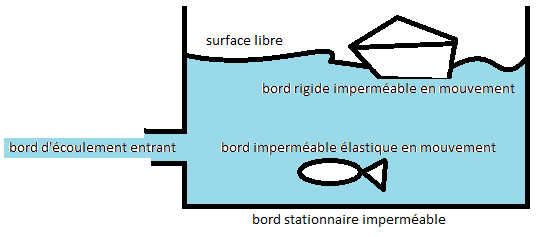
\includegraphics[scale=0.5]{bords.png}
\caption{\textit{Tous les bords possibles pour un fluide}}
\label{figure/boundaries}
\end{figure}

Une frontière en \textit{paroi solide} est l'ensemble des points de contact entre le fluide avec un solide. En terme de vélocité: le fluide ne doit pas pénétrer à travers la frontière solide ou en sortir s'il y est contenu, donc la composante normale de la vélocité à cet emplacement est nulle: $\overrightarrow{u}.\hat{n} = 0$ \newline
Cette équation s'applique surtout si le solide est statique. Dans le cas général ou la paroi est en mouvement, la composante normale de la vélocité du fluide doit correspondre à la composante normale de la vélocité du solide à son contact, c'est-à-dire:
	\begin{equation}
	\overrightarrow{u}.\hat{n} = \overrightarrow{u}\!	\!_{solid} \,.\, \hat{n}
	\end{equation}
$ \hat{n} $ est la normale à la frontière solide.
Ces équations représentent les conditions qui évitent au fluide de coller au solide, étant donné que la composante normale de la vélocité est restreinte, ce qui permet au fluide de glisser en suivant la direction tangentielle.
Sur cette frontière, la pression maintient le fluide dans son état \textit{incompressible} en préservant son volume et renforce les conditions sur la paroi solide.\newline 
Si le fluide était visqueux, les frottements provoqués par la viscosité auraient une influence sur la composante tangentielle de la vélocité du fluide. Le cas le plus simple est la condition de non-glissement de la frontière:
$\overrightarrow{u} = 0$ \newline
Si le solide est en mouvement, cette condition serait:
\begin{equation}
\overrightarrow{u} \,=\, \overrightarrow{u}\!\!_{solid}
\end{equation}
Parfois, le bord en paroi solide est un genre de drain que le fluide peut traverser. Dans ce cas, le produit $ \overrightarrow{u}\,.\,\hat{n} $ doit être différent de la vélocité au bord, et être plutôt égale à la vélocité d'aspiration ou de refoulement du conduit dans la simulation.

L'autre type de frontière est la \textit{surface libre} ou \textit{surface ouverte}. C'est l'ensemble des points où la modélisation du fluide n'est pas prise en compte. Par exemple, dans le cas de la simulation de l'eau, les surfaces de l'eau qui \textbf{ne sont pas} en contact avec les parois solides sont des surfaces libres. En réalité, l'eau est en contact avec un autre fluide qui est l'air, mais cela ajoute plus de complexité  pour ajouter la simulation de l'air dans l'équation. De plus, comme l'air est 700 fois plus léger que l'eau, il n'a pas un effet assez significatif sur l'eau. Donc, l'air est modélisé simplement comme étant une région avec une pression atmosphérique. Et puisque pour les fluides incompressibles, seules les \textbf{ différences} de pression comptent, la pression constante de l'air peut être choisi arbitrairement: zéro en l’occurrence. En conséquence, \textit{une surface ouverte est celle qui a une pression} $ p = 0 $, et la vélocité y est hors de contrôle.\newline
La surface ouverte est importante pour la simulation d'une petite partie de fluide faisant partie d'un domaine plus large: la simulation de la fumée dans l'air par exemple. Simuler l'atmosphère tout entier n'est pas envisageable, donc une limitation sur une grille qui englobe la "zone d'intérêt" est fixée pour la simulation. A la frontière de cette zone, le fluide doit continuer, mais la simulation ne dépasse pas cette limite. Seulement, comme la simulation laisse le fluide pénétrer ou sortir de cette zone, la frontière est considérée comme une surface ouverte, $ p = 0 $, même si il n'y a aucune surface visible.\newline
Pour les liquides de petites grandeurs, la tension à la surface peut être importante. Dans les couches intérieures moléculaires, la tension de surface existe à cause de la variation des forces d'attraction entre les molécules de différents types. Par exemple, les molécules d'eau sont fortement attirées plus par les autres molécules d'eau que par les molécules d'air: en conséquence, les molécules d'eau sur la surface séparant l'air et l'eau tendent à être entourés par encore plus d'eau que d'air. Sur le point de vue géométrique, les chimistes ont modélisé ce phénomène par l'action de forces cherchant à minimiser la surface, ou à réduire la courbure moyenne de la surface. En d'autres mots, c'est la tension qui essaye constamment à rétrécir la surface, d'où son nom de tension de surface. \newline

Les surfaces libres présentent un problème majeur: les bulles d'air se rompent immédiatement. Même si l'air est plus léger que l'eau, et qu'il ne peut pas transférer beaucoup d'élan à l'eau, il demeure incompressible. Une bulle d'air dans l'eau garde son volume. Modéliser une bulle d'air comme une surface ouverte provoquerait l'explosion de l'air. Pour pallier ce problème, il est possible de simuler en ajoutant des bulles d'air à la surface ouverte, ou plus généralement simuler l'air et l'eau (simulation à deux phases étant donné les deux fluides).



\section{La visualisation}

Les fluides ont été mathématiquement modélisés très largement depuis les années 50. Notamment, les travaux de  Harlow \cite{harlow-65} dans le groupe T3 de l'institut "Los Alamos National Laboratory" ont fourni des techniques pour la simulation des fluides telles que la structure de grille MAC (staggered marker-and-cell grid), la méthode PIC (Particle in Cell) qui a ouvert la voie vers les méthodes actuelles comme FLIP (Fluid-Implicit-Particle) ou MPM (Material Point Method).

Ces méthodes issues de la mécanique des fluides numériques (MFN) ne sont pas pratiques pour l'animation. Dans le domaine de la synthèse d'image, les deux grandes catégories de techniques les plus utilisées sont: les simulations \textbf{basées sur les grilles} et celles \textbf{basées sur les particules}. D'autres méthodes comme celle des réseaux de Boltzmann (LBM) ont été récemment introduites pour simuler des phénomènes physiques complexes comme les interactions chimiques entre les fluides. 
Les simulations basées sur les grilles sont très précises mais assez lentes tandis que celles basées sur les particules sont plus rapides mais donnent des résultats visuels moyens. Les techniques basées sur les grilles correspondent au point de vue d'Euler et facilitent les calculs de dérivées sur la grille, à l'opposé d'opérations compliquées sur un nuage de particules éparpillées. Et pour finir, ces méthodes donnent de bons résultats pour les surfaces lisses de l'eau par rapport à celles basées sur les particules.

\subsection{La grille d'Harlow}

Quelle est la place de la grille d'Harlow\cite{harlow-65} dans la simulation?  Il est nécessaire de stocker les grandeurs caractéristiques du fluide: la pression, la vélocité, la température, la concentration, etc. dans les différents points de l'espace. Ces valeurs sont alors disposées sur une grille. La grille d'Harlow combine une méthode de marquage de particules et une structure stockant les valeurs sur les différentes parties de la grille facilitant l'élaboration d'algorithmes efficaces.

La grille en dimension 2 est illustrée par la figure \ref{figure/2d-mac-grid}. La pression $p_{i,j}$ de la cellule $(i, j)$ est placée au centre de la cellule. La vélocité est décomposée en ses composantes cartésiennes: la composante horizontale $ u $ est basée sur les centres des faces verticales de la cellule. En l’occurrence, $ u_{i+1/2, j} $ indique la composante horizontale entre les cellules $(i, j)$ et $(i+1, j)$. La composante verticale de la vélocité est placée sur centres des faces horizontales de la cellule. Pour la cellule $(i, j)$ de la grille, la composante \textbf{normale} de la vitesse est placée au centre de chaque face de la cellule: cette disposition permet d'estimer naturellement la quantité de fluide entrante et sortante de la cellule. \newline

\begin{figure}[!htbp]
\centering
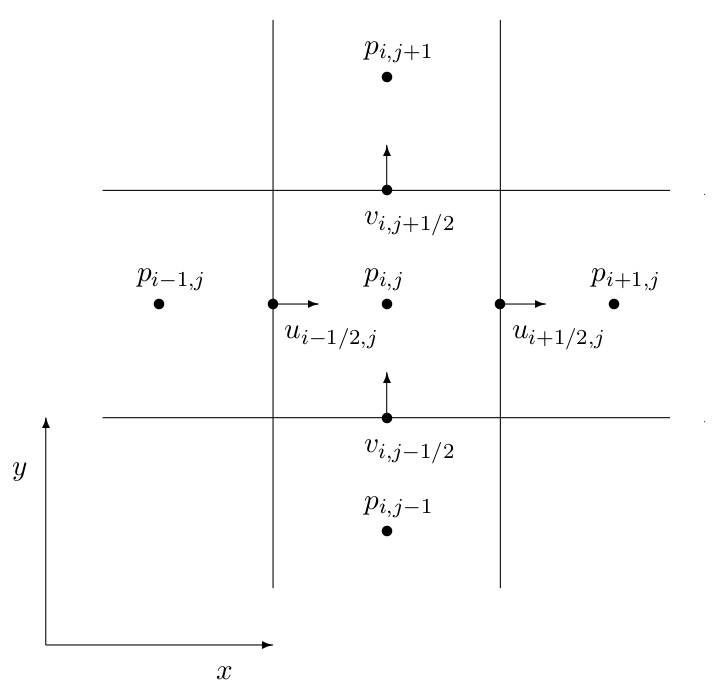
\includegraphics[scale=0.5]{2d-mac-grid.png}
\caption{\textit{Grille MAC en dimension 2: la pression est située au centre de la grille, la composante verticale de la vélocité est définie sur les faces horizontales des cellules et sa composante horizontale sur les faces verticales des cellules}}
\label{figure/2d-mac-grid}
\end{figure}

En dimension 3, la grille MAC est configurée de la même manière, la pression au centre de la cellule de la grille et les trois composantes de la vitesse sont décomposées de telle façon que la composante normale soit placée au centre de chaque face de la cellule, voir figure \ref{figure/3d-mac-grid}.\newline 
\begin{figure}[!htbp]
\centering
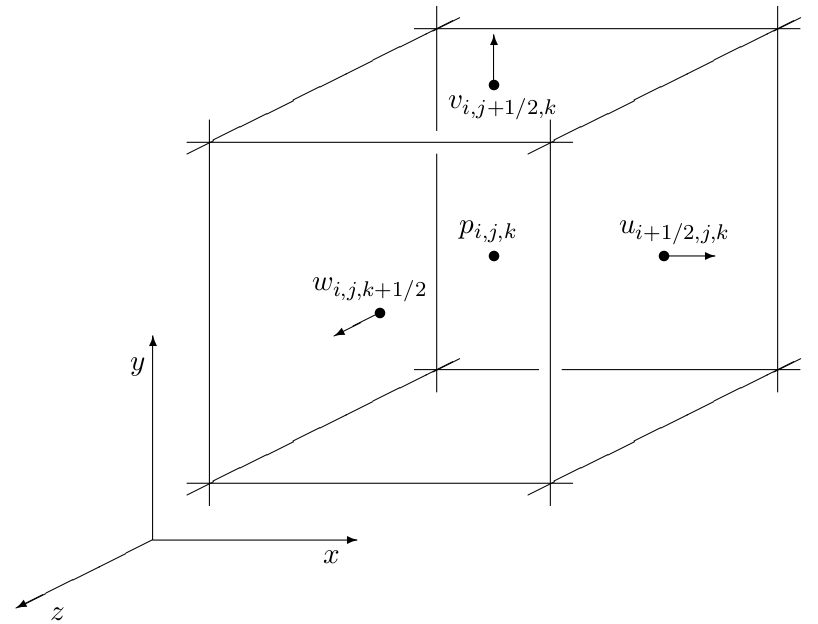
\includegraphics[scale=0.5]{3d-mac-grid.png}
\caption{\textit{Une cellule de la grille MAC en dimension 3}}
\label{figure/3d-mac-grid}
\end{figure}
Pour simplifier, la grille MAC est utilisée pour pouvoir utiliser les "\textbf{différences centrales}" du gradient de la pression et de la divergence du champ des vecteurs de vitesse sans les désavantages cette méthode.
\newpage
\subsection{De la stabilité de Stam au FLIP incompressible de Bridson}

Les premiers à avoir fait avancer la simulation des fluides incompressibles sont Nick Foster et Dimitris Metaxas \cite{Foster-96}. Avant eux, les méthodes pour animer l'eau reposaient sur la modélisation de l'interaction entre la lumière et l'eau pour réaliser des effets comme la réflexion, la réfraction sans prendre en compte les propriétés physiques de l'eau. \newline
La participation de Jos Stam \cite{stam-99} a été aussi déterminante pour l'avancé de la simulation des fluides. Jos Stam a introduit une méthode dite "semi-lagrangienne" qui rectifie une instabilité dans la méthode d'Euler pour la discrétisation du fluide dans une grille et a grandement amélioré la rapidité et l'efficacité de la simulation des fluides.

Les méthodes trouvées étaient alors stables et produisaient d'excellents résultats pour la simulation des fluides placides et sans perturbations, réalistes mais trop calmes pour simuler des situations plus chaotiques. La dissipation numérique était également excessive. Le mathématicien Stanley Joel Osher et son doctorant Ronald Fedkiw \cite{osher-fedkiw-2002} ont proposé la méthode des surfaces de niveau formées de surfaces implicites pour remplacer le système de maillage dans la numérisation du fluide. Les travaux d'Osher ont été poursuivi par Fedkiw qui a proposé une interpolation à plus haut degré et le confinement de la vorticité. Fedkiw a initié les méthodes concernant les surfaces complexes de l'eau, puis le doctorant Robert Bridon\footnote{Site web de Robert Bridson: \url{http://www.cs.ubc.ca/~rbridson/}. C'est un ancien chercheur en Mathématiques et en Imagerie de l'université "University of British Columbia" qui a travaillé sur de multiples simulations de fluides pour les effets spéciaux au cinéma dont le Hobbit, Avatar, Pirates des caraïbes 4, et également sur des logiciels de simulation pour les éditeurs comme Autodesk, et est en plus un des piliers du projet PhysBam pour les animations basées sur la Physique de l'Université de Stanford, USA.} sous la tutelle de ce dernier a suivi ses pas. Bridson a amélioré les anciennes méthodes d'Harlow pour les adapter à ses travaux sur les écoulements incompressibles introduisant par la même la méthode "FLIP incompressible" pour l'animation des fluides, très utilisée dans le cinéma d'animation comme Pipper \cite{serritella-2016} ou The good dinausor de Pixar\cite{reisch-2016}.

\section{La simulation de la fumée}

En considérant la fumée, selon l'article de Fedkiw et al. \cite{fedkiw-stam-jensen-01}, le fluide est l'air dans lequel des particules de fumée sont suspendues. Pour modéliser la fumée, deux variables du fluide supplémentaires sont nécessaires: la température $T$ de l'air et la concentration $s$ de particules de fumée, la partie visible.\newline
En réalité, des changements de température entrainent une expansion ou une contraction de l'air, changeant la densité. La masse de particules de fumée provoque aussi l'augmentation de la densité. Comme ces variations sont infimes, une approximation de "\textbf{Boussinesq}" est possible pour supposer une densité constante. De plus, la force de la gravité est remplacée par la force de flottaison \textit{$f_{buoy}$} qui est tirée de ces variations. Pour être plus pratique, la flottaison est supposée linéairement dépendante de la température et de la concentration de fumée uniquement. Soit $T_{amp}$ la température ambiante, par exemple 300K à Antananarivo, on prend comme force de flottaison:
\begin{equation}
f_{buoy} = (0, -\alpha s + \beta (T-T_{amb}) ,0)
\end{equation}
$\alpha$ et $\beta$ sont des constantes positives pouvant être choisies arbitrairement. La force $f_{buoy}$ est nulle s'il n'y a pas de fumée ou si la température correspond à la température ambiante.
$T$ et $s$ sont placés sur les centres des cellules la grille, au même titre que la pression. Pour ajouter la force de flottaison à la composante $v$ de la vélocité sur la grille MAC, il faut évaluer la moyenne des valeurs pour $T$ et $s$ par rapport à leurs centres voisins, par exemple $T_{i, j+1/2, k} = (T_{i,j,k} + T_{i,j+1,k})/2$.\newline
Les quantités $T$ et $s$ subissent une advection avec le fluide, elles sont également diffusées. Cependant, comme la viscosité est éliminée de l'équation étant de toute façon imitée par l'inévitable dissipation numérique, les nouvelles équations d'évolution sont simplement:
\begin{equation}
\frac{DT}{Dt} = 0 \,\,\,\,\,\,\, \frac{Ds}{Dt} = 0
\end{equation}

L'advection de la température et de la concentration de fumée sont réalisées de manière synchrone à celle de la vélocité.\newline
Les conditions aux bords pour la fumée sont simples. Pour la vélocité et la pression, les bords autour duquel la fumée tourne sont des bords solides, et dans les parties de la grille qui ne sont pas inclues le bord est formée d'une surface libre ($p=0$). Le champ de température à l'intérieur des objets peut être étendu en prenant la température actuelle de l'objet, et en dehors du domaine la température ambiante $T_{amb}$. La concentration de la fumée n'existe pas à l'intérieur des objets, sauf si elle est supposée être déversée d'un objet (avec une vélocité de bord non nulle), dans quel cas une valeur source pour la fumée contenue dans l'objet doit être choisie. Dans le cas contraire, une extrapolation de la concentration de la fumée dans l'objet est nécessaire. Pour la fumée à l'intérieur, la concentration de fumée est l'interpolation des valeurs extérieures les plus proches.\newline

La modélisation sur la grille présente des inconvénients après l'advection: les petites vorticités séparant l'air pure des particules de fumée disparaissent trop rapidement. Ce problème est dû à la dissipation numérique excessive.

\subsection{Le confinement}

Pour pallier le problème de vorticités disparaissant artificiellement trop vite, une force de "\textbf{confinement}" est ajoutée:
\begin{equation}
\overrightarrow{\omega} = \nabla \times \overrightarrow{u}
\end{equation}
$\nabla \times$ est l'opérateur différentiel "rotationnel". Pour une rotation rigide du champ de vélocités, la vorticité est exactement le double de la vitesse angulaire, d'où la mesure des caractéristiques rotationnelles. Un vortex, vaguement parlant, est un pic dans le champ de vorticité, une place qui tourbillonne plus vite que tout autre fluide aux alentours.\newline
Le champ de force a pour rôle d'accroître la vorticité, c'est le confinement de vorticité. L'astuce consiste à trouver la direction que cette force doit prendre pour accroitre la rotation d'un vortex.\newline
Où se trouvent les tourbillons (vortices): les maximales locales de vorticité? Il faut élaborer des vecteurs unitaires $\overrightarrow{N}$ qui pointent sur ces vorticités simplement en normalisant le gradient de $ |\overrightarrow{\omega}|$:
\begin{equation}
\overrightarrow{N} = \frac{\nabla |\overrightarrow{\omega}|}{\| \nabla |\overrightarrow{\omega}| \|}
\end{equation}
Maintenant, $\overrightarrow{N}$ pointe vers le centre de rotation d'un vortex, et $\overrightarrow{\omega}$ lui-même pointe le long de l'axe de rotation, donc pour obtenir un vecteur de force qui fait augmenter la rotation, il faut prendre le produit vectoriel:
\begin{equation}
f_{conf} = \epsilon \,\, \Delta x \,\, (\overrightarrow{N} \,\, \times \,\, \overrightarrow{\omega})
\end{equation}
$\epsilon$ est un paramètre pour contrôler l'effet du confinement de vorticité. Le terme $\Delta x$ est un coefficient de consistance.\newline
Pour l'implémentation numérique, il faut calcul d'abord les moyennes des vélocités sur la grille MAC avec les centres des cellules, et utiliser la dérivées centrales pour approximer la vorticité :
\begin{equation}
\overrightarrow{\omega}_{i,j,k} = 
	\left(
		\begin{array}{c}
			\frac{w_{i,j+1,k} - w_{i,j-1,k}}{2\,\Delta x} - \frac{v_{i,j,k+1} - v_{i,j,k-1}}{2\,\Delta x}, \\
			\frac{u_{i,j,k+1} - u_{i,j,k-1}}{2\,\Delta x} - \frac{w_{i+1,j,k} - w_{i-1,j,k}}{2\,\Delta x}, \\
	 		\frac{v_{i+1,j,k} - v_{i-1,j,k}}{2\,\Delta x} - \frac{u_{i,j+1,k} - u_{i,j-1,k}}{2\,\Delta x}
		\end{array}
	\right)
\end{equation}
Le gradient de |\overrightarrow{\omega}| est estimé similairement en utilisant les différences centrales aux centres des cellules de la grille, utilisées pour définir $\overrightarrow{N}$:
\begin{equation}
\nabla |\overrightarrow{\omega}| _{i,j,k} = 
	\left(
		\frac{|\overrightarrow{\omega}|_{i+1,j,k} - |\overrightarrow{\omega}|_{i-1,j,k} }{2 \,\Delta x},\,
		\frac{|\overrightarrow{\omega}|_{i,j+1,k} - |\overrightarrow{\omega}|_{i,j-1,k} }{2 \,\Delta x},\,
		\frac{|\overrightarrow{\omega}|_{i,j,k+1} - |\overrightarrow{\omega}|_{i,j,k-1} }{2 \,\Delta x}
 	\right)
\end{equation}
Il faut normaliser ce terme pour obtenir $N$, et éviter la division par zéro en utilisant, par exemple:
\begin{equation}
\overrightarrow{N}_{i,j,k} = \frac{\nabla |\overrightarrow{\omega}|_{i,j,k}}{\| \nabla |\overrightarrow{\omega}|_{i,j,k} \| + 10^{-20}}
\end{equation}
Finalement, pour obtenir $f_{conf}$ il faut prendre le produit vectoriel. \newline

En dimension 2, les composantes bidimensionnelles de la vélocité peuvent être considérées comme $(u,v,0)$. Cela donne un champ de vorticité $\overrightarrow{\omega} = (0,0,\omega)$, assimilable au scalaire $\omega$. \newline

La vorticité est un caractère extrêmement important pour les fluides. De nombreuses méthodes numériques pour l'écoulement des liquides ont été tirées de l'équation de vorticité, particulièrement en dimension 2 où elle est particulièrement simple. Généralement, ces méthodes pour la vorticité donnent précisément la localisation, la force, et l'axe des tourbillons. Mais en dimension 3, il est difficile de modéliser avec précision les interactions aux bords. Les travaux de Selle et al. \cite{Selle-2005} démontrent comment retracer les particules de voxels qui introduisent plus de précision dans une version du confinement de vorticité.

\section{Le rendu}

Un fluide évolue dans un espace en deux ou trois dimensions qui doit être discrétisé. Chaque cellule de la grille contient les valeurs des grandeurs caractéristiques de la grille. Particulièrement en dimension 3, ces cellules peuvent être des voxels. Pour afficher la simulation il faut utiliser les rendus volumiques. \newline
Il est possible de dessiner directement ces voxels sur l'écran, en positionnant sa projection sur l'écran et la couleur du résultat de cette projection. Mais cela est très couteux en termes de polygones mis en jeu.\newline
Un autre manière est d'utiliser des tranches grâce aux textures 3D pour afficher les données volumiques face à la caméra. La variation des tranches dessinées donnent des images lisses.\newline
Une troisième option est l'utilisation de lancer de rayons: un rayon traverse le cube du fluide et il faut calculer la couleur finale à partir des échantillons des voxels traversés. En notant que la couleur du rayon dans le fluide est proportionnelle à la transparence et l'épaisseur de celui-ci, les couleurs fortes correspondent à des rayons longs.

Donc il y a plusieurs façons de faire le rendu des fluides définis par des particules.\newline
Une des plus simples et des plus rapides de ces méthodes est l'utilisation de sprites. Grâce à l'application d'un filtre de lissage, les sprites sont dessinées sans la granularité sous un seuil défini. \newline
Une autre manière est de dessiner une isosurface du champ de masse volumique et de la triangulariser en utilisant le "Marching cube", c'est-à-dire pour chaque point il faut prendre les cubes qui l'entourent et déterminer ensuite les polygones nécessaires pour représenter l'isosurface.



\section{Conclusion}

La simulation des fluides est une pratique en tout temps utile directement pour simuler des fluides comme la fumée et l'eau. Utilisée en ingénierie pour tester les modélisations d'avions ou les réseaux de pipelines, et dans l'étude des flux automobiles sur les routes, la simulation des fluides fait partie des ingrédients nécessaires pour créer des environnements physiques réalistes. Le principal souci est la résolution ou plutôt l'approximation de la solution des équations physiques régissant les fluides, qui est couteuse en terme de calcul. De plus en plus d'algorithmes et de techniques sont mis en \oe uvre pour améliorer le résultat, comme la SPH (Smoothed Particle Hydrodynamics) \cite{muller-2003} pour la simulation en temps réel des jets d'eau et des phénomènes aquatiques complexes rencontrés dans les jeux vidéos et la réalité virtuelle ou l'exploitation des équations de Schr$\ddot{o}$dinger pour la simulation de fumée \cite{chern-2016}. Récemment même l'intelligence artificielle est mise à contribution pour la simulation des fluides comme l'utilisation des méthodes Random Forest \cite{ladicky-2015} pour gagner en rapidité. Le domaine de l'image de synthèse n'est pas en reste car de plus en plus d'animations ou d'effets visuels nécessitent une simulation de qualité capable de convaincre les yeux du téléspectateur.

\newpage
\begin{thebibliography}{2} 

\bibitem{chern-2016}
Albert CHERN, Felix KN$\ddot{O}$PPEL, Ulrich PINKALL, Peter SCHR$\ddot{O}$DER, and Steffen WEIßMANN. 2016.
\textit{Schr$\ddot{o}$dinger's smoke}.
 ACM Trans. Graph. 35, 4, Article 77 (July 2016), 13 pages. 

\bibitem{da-2016}
Fang DA, David HAHN, Christopher BATTY, Chris WOJTAN, and Eitan GRINSPUN. 2016.
\textit{Surface-only liquids}.
 ACM Trans. Graph. 35, 4, Article 78 (July 2016), 12 pages.

\bibitem{fedkiw-stam-jensen-01}
R. FEDKIW, J. STAM, and H. JENSEN. 2001.
\textit{Visual simulation of smoke}.
In Proc. SIGGRAPH, pages 15–22.

\bibitem{Foster-96}
Nick FOSTER and Dimitri METAXAS. 1996.
\textit{Realistic animation of liquids}.
Graph. Models Image Process. 58, 5, 471-483.

\bibitem{harlow-65}
F. HARLOW and J. WELCH. 1965.
\textit{Numerical Calculation of Time-Dependent Viscous Incompressible Flow of Fluid with Free Surface}.
Phys. Fluids, 8:2182–2189.

\bibitem{Hong-05}
Jeong-Mo HONG and Chang-Hun KIM. 2005.
\textit{Discontinuous fluids}.
ACM Trans. Graph. (Proc. SIGGRAPH),24:915–920.

\bibitem{ladicky-2015}
L'ubor LADICK\'{Y}, SoHyeon JEONG, Barbara SOLENTHALER, Marc POLLEFEYS, and Markus GROSS. 2015.
\textit{Data-driven fluid simulations using regression forests}.
ACM Trans. Graph. 34, 6, Article 199 (October 2015), 9 pages.

\bibitem{muller-2003}
Matthias M$\ddot{U}$LLER, David CHARYPAR, and Markus GROSS. 2003.
\textit{Particle-based fluid simulation for interactive applications}.
In Proceedings of the 2003 ACM SIGGRAPH/Eurographics symposium on Computer animation (SCA '03). Eurographics Association, Aire-la-Ville, Switzerland, Switzerland, 154-159.

\bibitem{osher-fedkiw-2002}
S. OSHER and R. FEDKIW. 2002.
\textit{Level Set Methods and Dynamic Implicit Surfaces}.
Springer-Verlag. New York, NY.

\bibitem{peer-2015}
Andreas PEER, Markus IHMSEN, Jens CORNELIS, and Matthias TESCHNER. 2015.
\textit{An implicit viscosity formulation for SPH fluids}.
ACM Trans. Graph. 34, 4, Article 114 (July 2015), 10 pages.

\bibitem{reisch-2016}
Jon REISCH, Stephen MARSHALL, Magnus WRENNINGE, Tolga GOKTEKIN, Michael HALL, Michael O'BRIEN, Jason JOHNSTON, Jordan REMPEL, and Andy LIN. 2016.
\textit{ Simulating rivers in the good dinosaur}.
 In ACM SIGGRAPH 2016 Talks (SIGGRAPH '16). ACM, New York, NY, USA, Article 40 , 1 pages

\bibitem{Selle-2005}
Andrew SELLE, Nick RASMUSSEN, and Ronald FEDKIW. 2005.
\textit{A vortex particle method for smoke, water and explosions}.
ACM Trans. Graph. (Proc. SIGGRAPH), pages 910–914.

\bibitem{serritella-2016}
Vincent SERRITELLA, Hosuk CHANG, Leon J. W. PARK, Ferdi SCHEEPERS, and Brett LEVIN. 2016.
\textit{Lapping water effects in Piper}.
In ACM SIGGRAPH 2016 Talks (SIGGRAPH '16). ACM, New York, NY, USA, Article 39 , 1 pages

\bibitem{stam-99}
Jos STAM. 1999.
\textit{Stable fluids}.
In Proc. SIGGRAPH, pages 121–128.

\end{thebibliography}

\end{document}